\documentclass[12pt,a4paper]{article}
\usepackage[utf8]{inputenc}
\usepackage[spanish]{babel}
\usepackage{geometry}
\usepackage{booktabs}
\usepackage{array}
\usepackage{enumitem}
\usepackage{graphicx}
\usepackage{xcolor}
\usepackage{needspace}

\title{Identificación de Riesgos}
\author{David Mato}
\date{\today}

\begin{document}
	\setcounter{tocdepth}{2}
	\maketitle
	
	\tableofcontents
	
	\section{Ejercicio 1}
	
	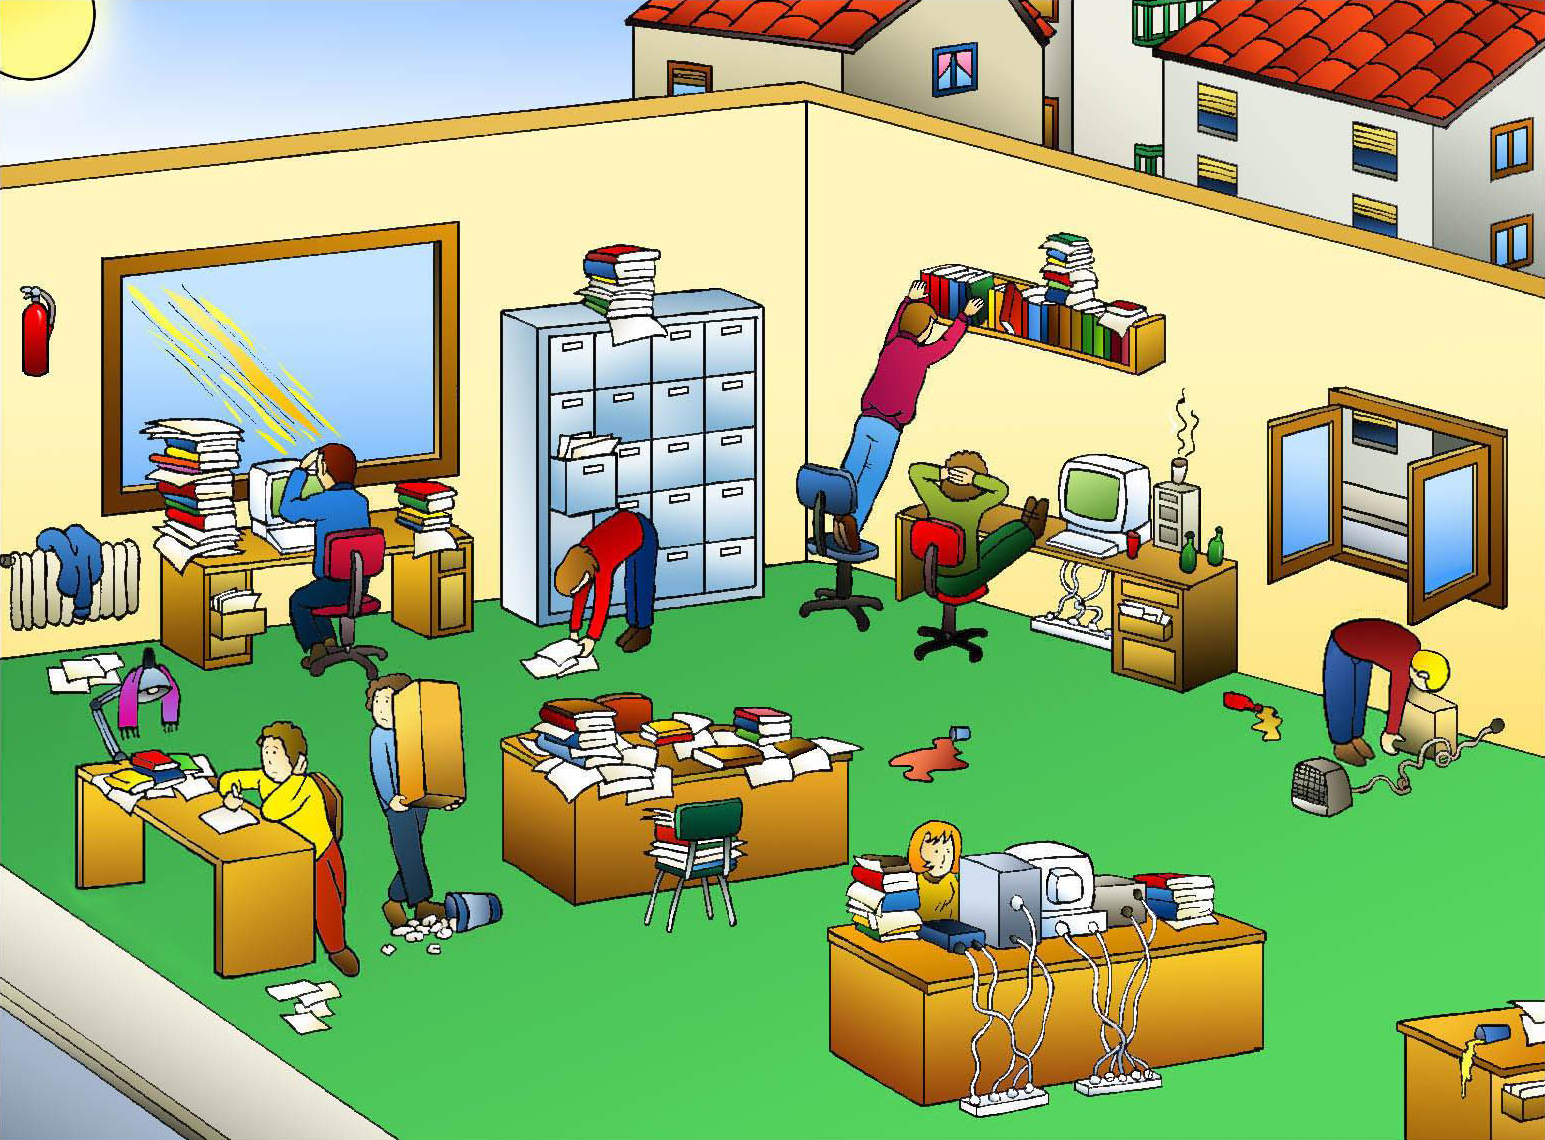
\includegraphics[width=0.9\textwidth]{../assignments/images/Identificación de Riesgos/01.jpg}
	
	\subsection{Persona 1 (Sentada de espaldas, ordenador - arriba izquierda)}
	\label{subsec:persona1} % Opcional
	
	\begin{itemize}
		\item \subsubsection{Riesgos Identificados}
		\begin{itemize}
			\item \textit{Posturas inadecuadas:} Posible mala postura frente al ordenador (espalda, cuello), reflejos en pantalla por la ventana.
			\item \textit{Contactos eléctricos:} Derivado del uso de equipos informáticos.
		\end{itemize}
		\subsubsection{Medidas a Adoptar}
		\begin{itemize}
			\item Evaluación ergonómica del puesto (silla, pantalla, reposapiés).
			\item Instalar persianas/cortinas para evitar reflejos.
			\item Fomentar pausas activas y formación postural.
			\item Revisión periódica de instalación eléctrica y equipos.
		\end{itemize}
		\subsubsection{Nivel de Riesgo}
		\begin{itemize}
			\item Posturas inadecuadas: \textbf{Medio}
			\item Contactos eléctricos: \textbf{Bajo}
		\end{itemize}
	\end{itemize}
	
	\hrulefill
	
	\subsection{Persona 2 (Sentada escribiendo - centro izquierda)}
	\label{subsec:persona2} % Opcional
	
	\begin{itemize}
		\item \subsubsection{Riesgos Identificados}
		\begin{itemize}
			\item \textit{Posturas inadecuadas:} Por desorden, limitación de espacio, espalda curvada.
			\item \textit{Caída de objetos por desplome:} Pilas de papeles/libros inestables.
			\item \textit{Golpes contra objetos inmóviles:} Acumulación de objetos en la mesa.
		\end{itemize}
		\subsubsection{Medidas a Adoptar}
		\begin{itemize}
			\item Política de orden y limpieza ("Clean Desk").
			\item Mobiliario adecuado (silla, mesa).
			\item Formación en higiene postural.
			\item Uso de estanterías/archivadores.
		\end{itemize}
		\subsubsection{Nivel de Riesgo}
		\begin{itemize}
			\item Posturas inadecuadas: \textbf{Medio}
			\item Caída de objetos por desplome: \textbf{Bajo}
			\item Golpes contra objetos inmóviles: \textbf{Bajo}
		\end{itemize}
	\end{itemize}
	
	\hrulefill
	
	\subsection{Persona 3 (Transportando caja - centro izquierda, de pie)}
	\label{subsec:persona3} % Opcional
	
	\begin{itemize}
		\item \subsubsection{Riesgos Identificados}
		\begin{itemize}
			\item \textit{Sobreesfuerzos:} Por peso/volumen de la caja.
			\item \textit{Caída de personas al mismo nivel:} Obstáculos en el suelo (papeles, líquido).
			\item \textit{Pisadas sobre objetos:} Papeles y objetos en el suelo.
			\item \textit{Caída de objetos en manipulación:} La propia caja.
		\end{itemize}
		\subsubsection{Medidas a Adoptar}
		\begin{itemize}
			\item Uso de medios mecánicos (carritos).
			\item Mantener zonas de paso despejadas.
			\item Formación en manipulación manual de cargas.
			\item Uso de calzado adecuado.
		\end{itemize}
		\subsubsection{Nivel de Riesgo}	
	\end{itemize}
	
	\hrulefill
	
	\subsection{Persona 4 (Sentada, ordenador, cables suelo - abajo centro)}
	\label{subsec:persona4} % Opcional
	
	\begin{itemize}
		\item \subsubsection{Riesgos Identificados}
		\begin{itemize}
			\item \textit{Contactos eléctricos:} Cables desorganizados/deteriorados en el suelo.
			\item \textit{Caída de personas al mismo nivel:} Tropiezo con cables.
			\item \textit{Posturas inadecuadas:} Posición frente al ordenador.
			\item \textit{Caída de objetos por desplome:} Pila de libros inestable.
		\end{itemize}
		\subsubsection{Medidas a Adoptar}
		\begin{itemize}
			\item Organizar y proteger cableado (canaletas, regletas fijas).
			\item Revisión periódica de cables y enchufes.
			\item Evaluación ergonómica del puesto.
			\item Ordenar y almacenar documentos/libros.
		\end{itemize}
		\subsubsection{Nivel de Riesgo}
		\begin{itemize}
			\item Contactos eléctricos: \textbf{Medio}
			\item Caída de personas al mismo nivel: \textbf{Medio}
			\item Posturas inadecuadas: \textbf{Bajo-Medio}
			\item Caída de objetos por desplome: \textbf{Bajo}
		\end{itemize}
	\end{itemize}
	
	\hrulefill
	
	\subsection{Persona 5 (Subida en silla - arriba centro)}
	\label{subsec:persona5} % Opcional
	
	\begin{itemize}
		\item \subsubsection{Riesgos Identificados}
		\begin{itemize}
			\item \textit{Caída de personas a distinto nivel:} Uso de silla inestable como escalera.
			\item \textit{Caída de objetos en manipulación:} Libros que intenta alcanzar.
			\item \textit{Caída de objetos por desplome:} Libros de la estantería.
			\item \textit{Golpes contra objetos inmóviles:} Al caer.
			\item \textit{Sobreesfuerzos:} Postura forzada.
		\end{itemize}
		\subsubsection{Medidas a Adoptar}
		\begin{itemize}
			\item Prohibición de subirse al mobiliario.
			\item Proporcionar escaleras manuales homologadas.
			\item Formación sobre uso seguro de equipos.
			\item Reorganizar almacenamiento (objetos frecuentes a mano).
		\end{itemize}
		\subsubsection{Nivel de Riesgo}
		\begin{itemize}
			\item Caída de personas a distinto nivel: \textbf{Alto}
			\item Caída de objetos (manipulación/desplome): \textbf{Medio}
			\item Golpes contra objetos inmóviles: \textbf{Medio}
			\item Sobreesfuerzos: \textbf{Bajo-Medio}
		\end{itemize}
	\end{itemize}
	
	\hrulefill
	
	\subsection{Persona 6 (Relajado, pies en mesa - arriba centro)}
	\label{subsec:persona6} % Opcional
	
	\begin{itemize}
		\item \subsubsection{Riesgos Identificados}
		\begin{itemize}
			\item \textit{Caída de personas al mismo nivel:} Desequilibrio de la silla.
			\item \textit{Posturas inadecuadas:} Postura forzada no ergonómica.
			\item \textit{Contactos eléctricos:} Equipos informáticos antiguos.
			\item \textit{Contactos térmicos:} Generación de calor por monitor antiguo.
		\end{itemize}
		\subsubsection{Medidas a Adoptar}
		\begin{itemize}
			\item Instruir sobre uso correcto del mobiliario.
			\item Fomentar posturas adecuadas.
			\item Asegurar estabilidad de las sillas (normativa).
			\item Revisar/renovar equipos eléctricos antiguos.
		\end{itemize}
		\subsubsection{Nivel de Riesgo}
		\begin{itemize}
			\item Caída de personas al mismo nivel: \textbf{Medio}
			\item Posturas inadecuadas: \textbf{Bajo-Medio}
			\item Contactos eléctricos: \textbf{Bajo}
			\item Contactos térmicos: \textbf{Bajo}
		\end{itemize}
	\end{itemize}
	
	\hrulefill
	
	\subsection{Persona 7 (Recogiendo papeles - centro, junto archivador)}
	\label{subsec:persona7} % Opcional
	
	\begin{itemize}
		\item \subsubsection{Riesgos Identificados}
		\begin{itemize}
			\item \textit{Posturas inadecuadas:} Flexión excesiva de espalda.
			\item \textit{Sobreesfuerzos:} Movimiento al agacharse/levantarse.
			\item \textit{Golpes contra objetos inmóviles:} Al incorporarse.
			\item \textit{Pisadas sobre objetos:} Sobre los papeles.
		\end{itemize}
		\subsubsection{Medidas a Adoptar}
		\begin{itemize}
			\item Formación en higiene postural (flexionar rodillas).
			\item Fomentar orden y limpieza.
			\item Realizar pausas si la tarea es repetitiva.
		\end{itemize}
		\subsubsection{Nivel de Riesgo}
		\begin{itemize}
			\item Posturas inadecuadas: \textbf{Medio}
			\item Sobreesfuerzos: \textbf{Medio}
			\item Golpes contra objetos inmóviles: \textbf{Bajo}
			\item Pisadas sobre objetos: \textbf{Bajo}
		\end{itemize}
	\end{itemize}
	
	\hrulefill
	
	\subsection{Persona 8 (Agachado, enchufe/calefactor - derecha)}
	\label{subsec:persona8} % Opcional
	
	\begin{itemize}
		\item \subsubsection{Riesgos Identificados}
		\begin{itemize}
			\item \textit{Contactos eléctricos:} Manipulación cerca de líquido derramado.
			\item \textit{Incendios:} Calefactor cerca de papeles/líquido.
			\item \textit{Contactos térmicos:} Quemadura con calefactor.
			\item \textit{Caída de personas al mismo nivel:} Líquido derramado.
			\item \textit{Posturas inadecuadas:} Posición forzada.
			\item \textit{Golpes contra objetos inmóviles:} Al moverse.
		\end{itemize}
		\subsubsection{Medidas a Adoptar}
		\begin{itemize}
			\item Acción inmediata Limpiar/secar líquido. Desconectar aparato (con seguridad).
			\item Alejar aparatos eléctricos de combustibles y líquidos.
			\item No manipular aparatos eléctricos cerca de líquidos/manos mojadas.
			\item Revisión de instalación y aparatos. Prohibir aparatos defectuosos.
			\item Formación sobre riesgo eléctrico y de incendios.
			\item Mantener suelos secos y despejados.
		\end{itemize}
		\subsubsection{Nivel de Riesgo}
		\begin{itemize}
			\item Contactos eléctricos: \textbf{Alto}
			\item Incendios: \textbf{Alto}
			\item Contactos térmicos: \textbf{Medio}
			\item Caída de personas al mismo nivel: \textbf{Medio}
			\item Posturas inadecuadas: \textbf{Bajo-Medio}
			\item Golpes contra objetos inmóviles: \textbf{Bajo}
		\end{itemize}
	\end{itemize}
	
	\hrulefill
	
	\section{Ejercicio 2}
	
	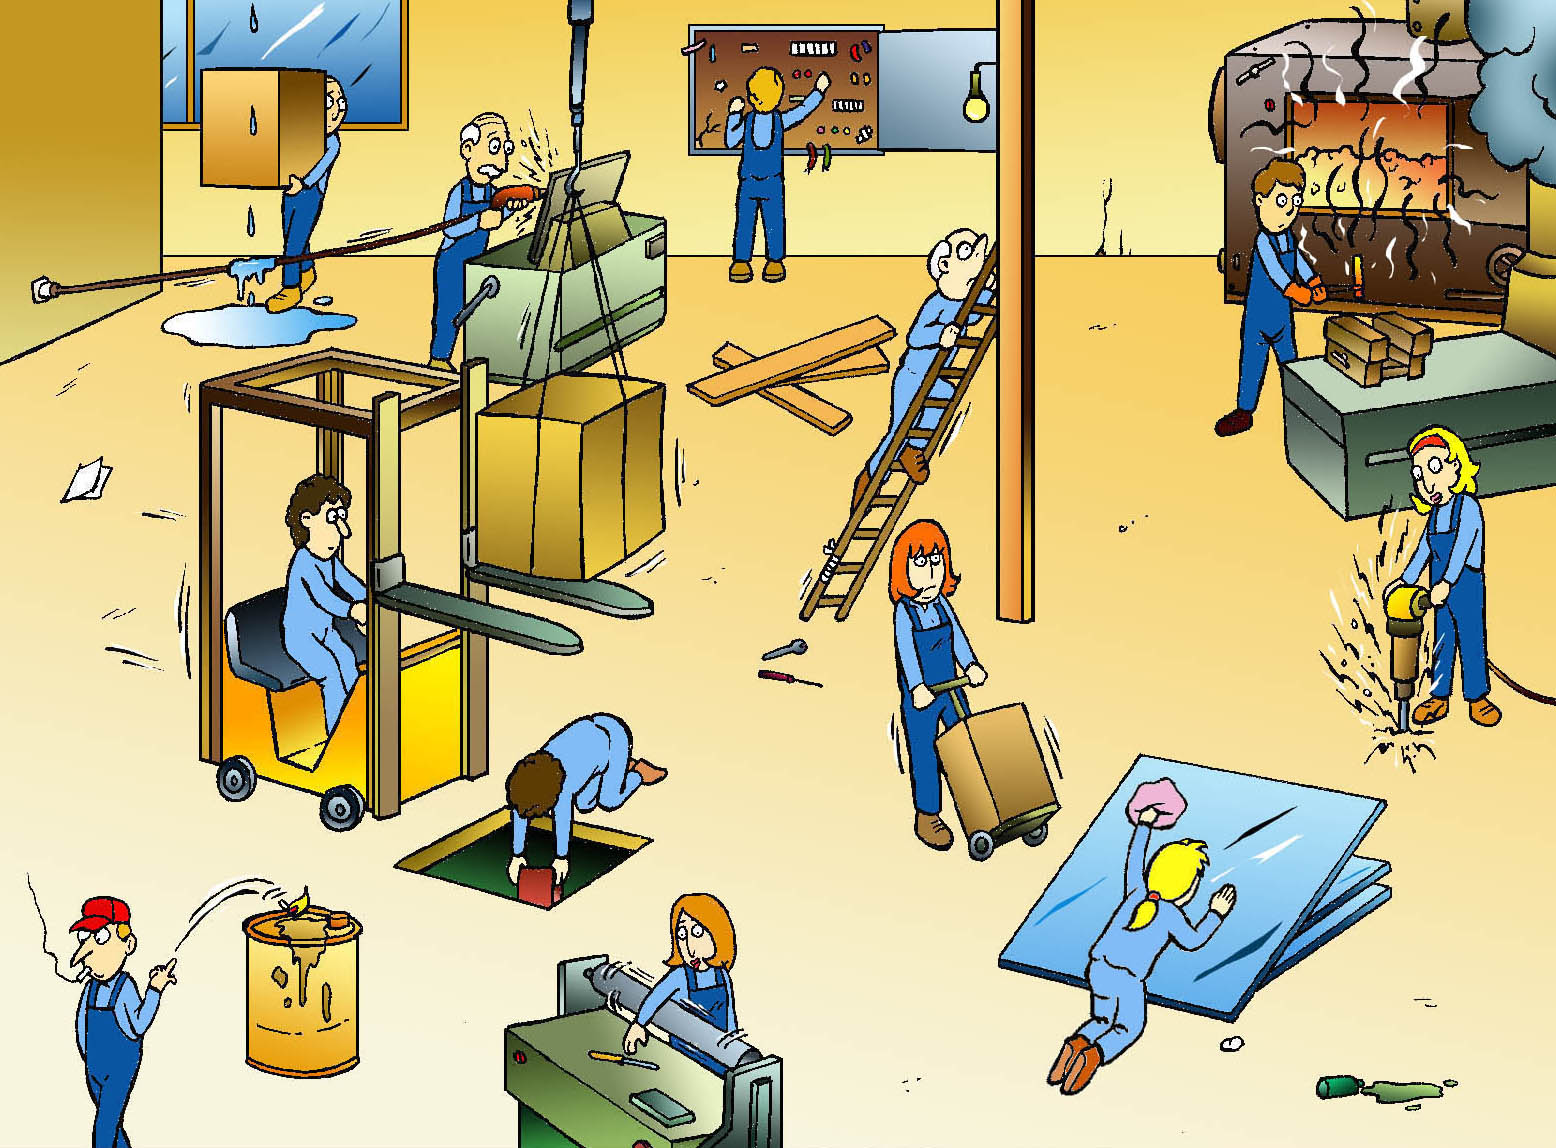
\includegraphics[width=0.9\textwidth]{../assignments/images/Identificación de Riesgos/02.jpg}
	
	\subsection{Persona 1 (Cargando caja, cerca de derrame - arriba izquierda)}
	
	\subsubsection{Riesgos Identificados}
	\begin{itemize}
		\item \textit{Caída de personas al mismo nivel:} Líquido derramado, barra metálica en el suelo.
		\item \textit{Pisadas sobre objetos:} Barra metálica.
		\item \textit{Sobreesfuerzos:} Manipulación manual de la caja.
		\item \textit{Caída de objetos en manipulación:} La caja que transporta.
	\end{itemize}
	
	\subsubsection{Medidas a Adoptar}
	\begin{itemize}
		\item Limpieza inmediata de derrames.
		\item Mantener pasillos y zonas de paso despejadas (retirar barra).
		\item Uso de medios auxiliares (carritos) si la carga es pesada/voluminosa.
		\item Formación en manipulación manual de cargas.
		\item Uso de calzado de seguridad (antideslizante).
	\end{itemize}
	
	\subsubsection{Nivel de Riesgo}
	\begin{itemize}
		\item Caída personas mismo nivel: \textbf{Medio}
		\item Pisadas sobre objetos: \textbf{Medio}
		\item Sobreesfuerzos: \textbf{Bajo-Medio}
		\item Caída objetos manipulación: \textbf{Bajo-Medio}
	\end{itemize}
	
	\bigskip\hrulefill\bigskip
	
	\subsection{Persona 2 (Operando carretilla elevadora - izquierda, centro)}
	
	\subsubsection{Riesgos Identificados}
	\begin{itemize}
		\item \textit{Atrapamientos por o entre objetos:} Para la Persona 3 si baja la carga.
		\item \textit{Caída de objetos por desplome:} Carga elevada inestable.
		\item \textit{Golpes contra objetos inmóviles:} Con estructuras u otros objetos.
		\item \textit{Caída de personas al mismo nivel:} Atropello de otros trabajadores.
	\end{itemize}
	
	\subsubsection{Medidas a Adoptar}
	\begin{itemize}
		\item Formación y autorización específica para carretilleros ("carnet de carretillero").
		\item \textbf{Prohibición absoluta} de situarse bajo cargas suspendidas.
		\item Asegurar y estabilizar la carga antes de elevarla/moverla.
		\item Mantener distancias de seguridad, usar señales acústicas/luminosas.
		\item Delimitar zonas de operación de carretillas.
	\end{itemize}
	
	\subsubsection{Nivel de Riesgo}
	\begin{itemize}
		\item Atrapamientos (para P3): \textbf{Alto}
		\item Caída objetos desplome: \textbf{Medio}
		\item Golpes contra objetos inmóviles: \textbf{Bajo-Medio}
		\item Caída personas mismo nivel (atropello): \textbf{Bajo-Medio}
	\end{itemize}
	
	\bigskip\hrulefill\bigskip
	
	\subsection{Persona 3 (Bajo carga suspendida - izquierda, abajo)}
	
	\subsubsection{Riesgos Identificados}
	\begin{itemize}
		\item \textit{Atrapamientos por o entre objetos / Caída de objetos por desplome:} Aplastamiento por la carga de la carretilla.
		\item \textit{Caída de personas a distinto nivel:} Al entrar/salir del foso/abertura.
		\item \textit{Golpes contra objetos inmóviles:} Bordes del foso, carretilla.
		\item \textit{Posturas inadecuadas:} Al trabajar en el foso.
	\end{itemize}
	
	\subsubsection{Medidas a Adoptar}
	\begin{itemize}
		\item Detener la operación inmediatamente.
		\item \textbf{Prohibición absoluta } de situarse o pasar bajo cargas suspendidas.
		\item Señalizar y proteger físicamente (barandillas, tapas resistentes) las aberturas en el suelo.
		\item Planificación de tareas: no realizar trabajos incompatibles simultáneamente.
		\item Procedimientos para trabajos en espacios confinados/fosos si aplica.
		\item Uso de casco.
	\end{itemize}
	
	\subsubsection{Nivel de Riesgo}
	\begin{itemize}
		\item Atrapamientos / Caída objetos desplome: \textbf{Muy Alto}
		\item Caída personas distinto nivel: \textbf{Alto}
		\item Golpes contra objetos inmóviles: \textbf{Bajo-Medio}
		\item Posturas inadecuadas: \textbf{Bajo-Medio}
	\end{itemize}
	
	\bigskip\hrulefill\bigskip
	
	\subsection{Persona 4 (Usando amoladora/similar - centro, arriba)}
	
	\subsubsection{Riesgos Identificados}
	\begin{itemize}
		\item \textit{Proyección de fragmentos o partículas:} Chispas, trozos de metal/muela.
		\item \textit{Incendios:} Chispas cerca de posibles materiales combustibles.
		\item \textit{Contactos térmicos:} Chispas, pieza caliente.
		\item \textit{Posturas inadecuadas:} Dependiendo de la posición de trabajo.
	\end{itemize}
	
	\subsubsection{Medidas a Adoptar}
	\begin{itemize}
		\item Uso obligatorio de EPIs: gafas/pantalla facial, guantes resistentes, ropa de trabajo adecuada (no sintética), protección auditiva si genera ruido.
		\item Instalar pantallas de protección colectiva.
		\item Retirar materiales combustibles o inflamables de la zona de trabajo.
		\item Verificar estado de la herramienta y discos.
		\item Permisos de trabajo en caliente si aplica.
	\end{itemize}
	
	\subsubsection{Nivel de Riesgo}
	\begin{itemize}
		\item Proyección fragmentos/partículas: \textbf{Alto}
		\item Incendios: \textbf{Medio-Alto} (depende del entorno)
		\item Contactos térmicos: \textbf{Medio}
		\item Posturas inadecuadas: \textbf{Bajo}
	\end{itemize}
	
	\bigskip\hrulefill\bigskip
	
	\subsection{Persona 5 (Subiendo escalera - centro)}
	
	\subsubsection{Riesgos Identificados}
	\begin{itemize}
		\item \textit{Caída de personas a distinto nivel:} Escalera dañada (peldaño roto), mal apoyada/inestable, sin sujeción.
		\item \textit{Caída de objetos en manipulación:} Si sube con herramientas/material.
		\item \textit{Golpes contra objetos inmóviles:} Al caer.
	\end{itemize}
	
	\subsubsection{Medidas a Adoptar}
	\begin{itemize}
		\item Revisión periódica de escaleras: retirar y señalizar las defectuosas.
		\item Uso de escaleras adecuadas, homologadas y en buen estado.
		\item Asegurar la estabilidad: apoyo firme, ángulo correcto (aprox. 75º), sujeción superior si es posible, base antideslizante.
		\item Formación sobre uso seguro de escaleras de mano (regla de los 3 puntos de apoyo).
		\item No transportar cargas pesadas/voluminosas al subir/bajar.
	\end{itemize}
	
	\subsubsection{Nivel de Riesgo}
	\begin{itemize}
		\item Caída personas distinto nivel: \textbf{Alto}
		\item Caída objetos manipulación: \textbf{Bajo-Medio}
		\item Golpes contra objetos inmóviles: \textbf{Bajo-Medio}
	\end{itemize}
	
	\bigskip\hrulefill\bigskip
	
	\subsection{Persona 6 (Empujando carrito - centro, abajo)}
	
	\subsubsection{Riesgos Identificados}
	\begin{itemize}
		\item \textit{Pisadas sobre objetos:} Herramienta (martillo) en el suelo.
		\item \textit{Caída de personas al mismo nivel:} Tropiezo con herramienta.
		\item \textit{Sobreesfuerzos:} Si la carga es excesiva o el carrito funciona mal.
		\item \textit{Golpes contra objetos inmóviles:} Con la herramienta, otros objetos, el propio carrito.
	\end{itemize}
	
	\subsubsection{Medidas a Adoptar}
	\begin{itemize}
		\item Política estricta de orden y limpieza: no dejar herramientas/materiales en zonas de paso.
		\item Mantenimiento preventivo de los carritos.
		\item Formación en manipulación de cargas / uso de carritos.
		\item Empujar en lugar de tirar de cargas pesadas siempre que sea posible.
	\end{itemize}
	
	\subsubsection{Nivel de Riesgo}
	\begin{itemize}
		\item Pisadas sobre objetos: \textbf{Medio}
		\item Caída personas mismo nivel: \textbf{Medio}
		\item Sobreesfuerzos: \textbf{Bajo-Medio}
		\item Golpes contra objetos inmóviles: \textbf{Bajo}
	\end{itemize}
	
	\bigskip\hrulefill\bigskip
	
	\subsection{Persona 7 (Cerca de horno - derecha, arriba)}
	
	\subsubsection{Riesgos Identificados}
	\begin{itemize}
		\item \textit{Contactos térmicos:} Radiación del horno, manipulación de piezas incandescentes sin protección adecuada.
		\item \textit{Proyección de fragmentos o partículas:} Salpicaduras de metal fundido, rotura de piezas calientes.
		\item \textit{Incendios:} Fuente de calor intensa, material incandescente.
		\item \textit{Posturas inadecuadas / Sobreesfuerzos:} Al manipular piezas.
	\end{itemize}
	
	\subsubsection{Medidas a Adoptar}
	\begin{itemize}
		\item Uso obligatorio de EPIs específicos para alta temperatura: guantes térmicos largos, traje/mandil ignífugo, polainas, pantalla facial.
		\item Instalar pantallas o barreras de protección contra radiación/proyecciones.
		\item Procedimientos de trabajo seguros y específicos para la tarea.
		\item Señalización clara de zonas con riesgo térmico.
		\item Formación específica.
	\end{itemize}
	
	\subsubsection{Nivel de Riesgo}
	\begin{itemize}
		\item Contactos térmicos: \textbf{Alto}
		\item Proyección fragmentos/partículas: \textbf{Medio-Alto}
		\item Incendios: \textbf{Medio}
		\item Posturas inadecuadas / Sobreesfuerzos: \textbf{Medio}
	\end{itemize}
	
	\bigskip\hrulefill\bigskip
	
	\subsection{Persona 8 (Usando martillo neumático - derecha, centro)}
	
	\subsubsection{Riesgos Identificados}
	\begin{itemize}
		\item \textit{Proyección de fragmentos o partículas:} Escombros, trozos de material.
		\item \textit{Atrapamientos por o entre objetos:} Derrumbe del material trabajado.
		\item \textit{Sobreesfuerzos / Posturas inadecuadas:} Peso y vibración de la herramienta.
		\item \textit{Caída de personas al mismo nivel:} Tropiezo con escombros.
		\item \textit{Golpes contra objetos inmóviles:} Con la herramienta, escombros.
		\item (\textit{Riesgos adicionales no listados: Exposición a Ruido y Vibraciones}).
	\end{itemize}
	
	\subsubsection{Medidas a Adoptar}
	\begin{itemize}
		\item Uso obligatorio de EPIs: gafas de seguridad/pantalla, protección auditiva, guantes antivibración, calzado de seguridad, casco si hay riesgo de caída de objetos.
		\item Delimitar y señalizar la zona de trabajo.
		\item Asegurar la estabilidad del elemento sobre el que se trabaja.
		\item Rotación de tareas y pausas para limitar exposición a vibraciones.
		\item Formación sobre manejo seguro y posturas.
		\item Mantenimiento de la herramienta.
	\end{itemize}
	
	\subsubsection{Nivel de Riesgo}
	\begin{itemize}
		\item Proyección fragmentos/partículas: \textbf{Alto}
		\item Atrapamientos: \textbf{Medio}
		\item Sobreesfuerzos / Posturas inadecuadas: \textbf{Medio}
		\item Caída personas mismo nivel: \textbf{Medio}
		\item Golpes contra objetos inmóviles: \textbf{Bajo-Medio}
		\item (\textit{Ruido/Vibraciones: Alto si no hay control})
	\end{itemize}
	
	\bigskip\hrulefill\bigskip
	
	\subsection{Persona 9 (Transportando planchas, tropieza - derecha, abajo)}
	
	\subsubsection{Riesgos Identificados}
	\begin{itemize}
		\item \textit{Caída de personas al mismo nivel:} Tropiezo con herramientas/escombros.
		\item \textit{Pisadas sobre objetos:} Herramientas/escombros.
		\item \textit{Caída de objetos en manipulación:} Las planchas metálicas.
		\item \textit{Sobreesfuerzos:} Peso y volumen de las planchas.
		\item \textit{Golpes contra objetos inmóviles:} Al caer, con las planchas.
		\item (\textit{Riesgo adicional no listado: Cortes con los bordes de las planchas}).
	\end{itemize}
	
	\subsubsection{Medidas a Adoptar}
	\begin{itemize}
		\item Mantener zonas de paso y trabajo limpias y ordenadas \textbf{rigurosamente}.
		\item Utilizar medios auxiliares (carros específicos, ventosas) para transportar planchas.
		\item Formación en manipulación manual de cargas.
		\item Uso obligatorio de EPIs: guantes anticorte, calzado de seguridad.
		\item Transporte entre dos personas si es necesario.
	\end{itemize}
	
	\subsubsection{Nivel de Riesgo}
	\begin{itemize}
		\item Caída personas mismo nivel: \textbf{Alto}
		\item Pisadas sobre objetos: \textbf{Medio}
		\item Caída objetos manipulación: \textbf{Medio}
		\item Sobreesfuerzos: \textbf{Medio}
		\item Golpes contra objetos inmóviles: \textbf{Medio}
		\item (\textit{Cortes: Medio-Alto si no usa guantes})
	\end{itemize}
	
	\bigskip\hrulefill\bigskip
	
	\subsection{Persona 10 (Fumando cerca de barril - izquierda, abajo)}
	
	\subsubsection{Riesgos Identificados}
	\begin{itemize}
		\item \textit{Incendios / Explosión:} Fuente de ignición (cigarrillo) cerca de barril con símbolo de inflamable.
		\item \textit{Contactos térmicos:} Quemadura por la colilla o el posible fuego.
	\end{itemize}
	
	\subsubsection{Medidas a Adoptar}
	\begin{itemize}
		\item \textbf{Prohibición estricta y señalizada} de fumar en todas las áreas de trabajo, especialmente cerca de sustancias inflamables.
		\item Almacenamiento seguro y señalizado de productos inflamables.
		\item Habilitar zonas específicas para fumadores, seguras y alejadas de riesgos.
		\item Formación y concienciación sobre el riesgo de incendio y explosión.
		\item Vigilancia y aplicación de sanciones por incumplimiento.
	\end{itemize}
	
	\subsubsection{Nivel de Riesgo}
	\begin{itemize}
		\item Incendios / Explosión: \textbf{Muy Alto}
		\item Contactos térmicos: \textbf{Bajo}
	\end{itemize}
	
	\section{Ejercicio 7}
	
	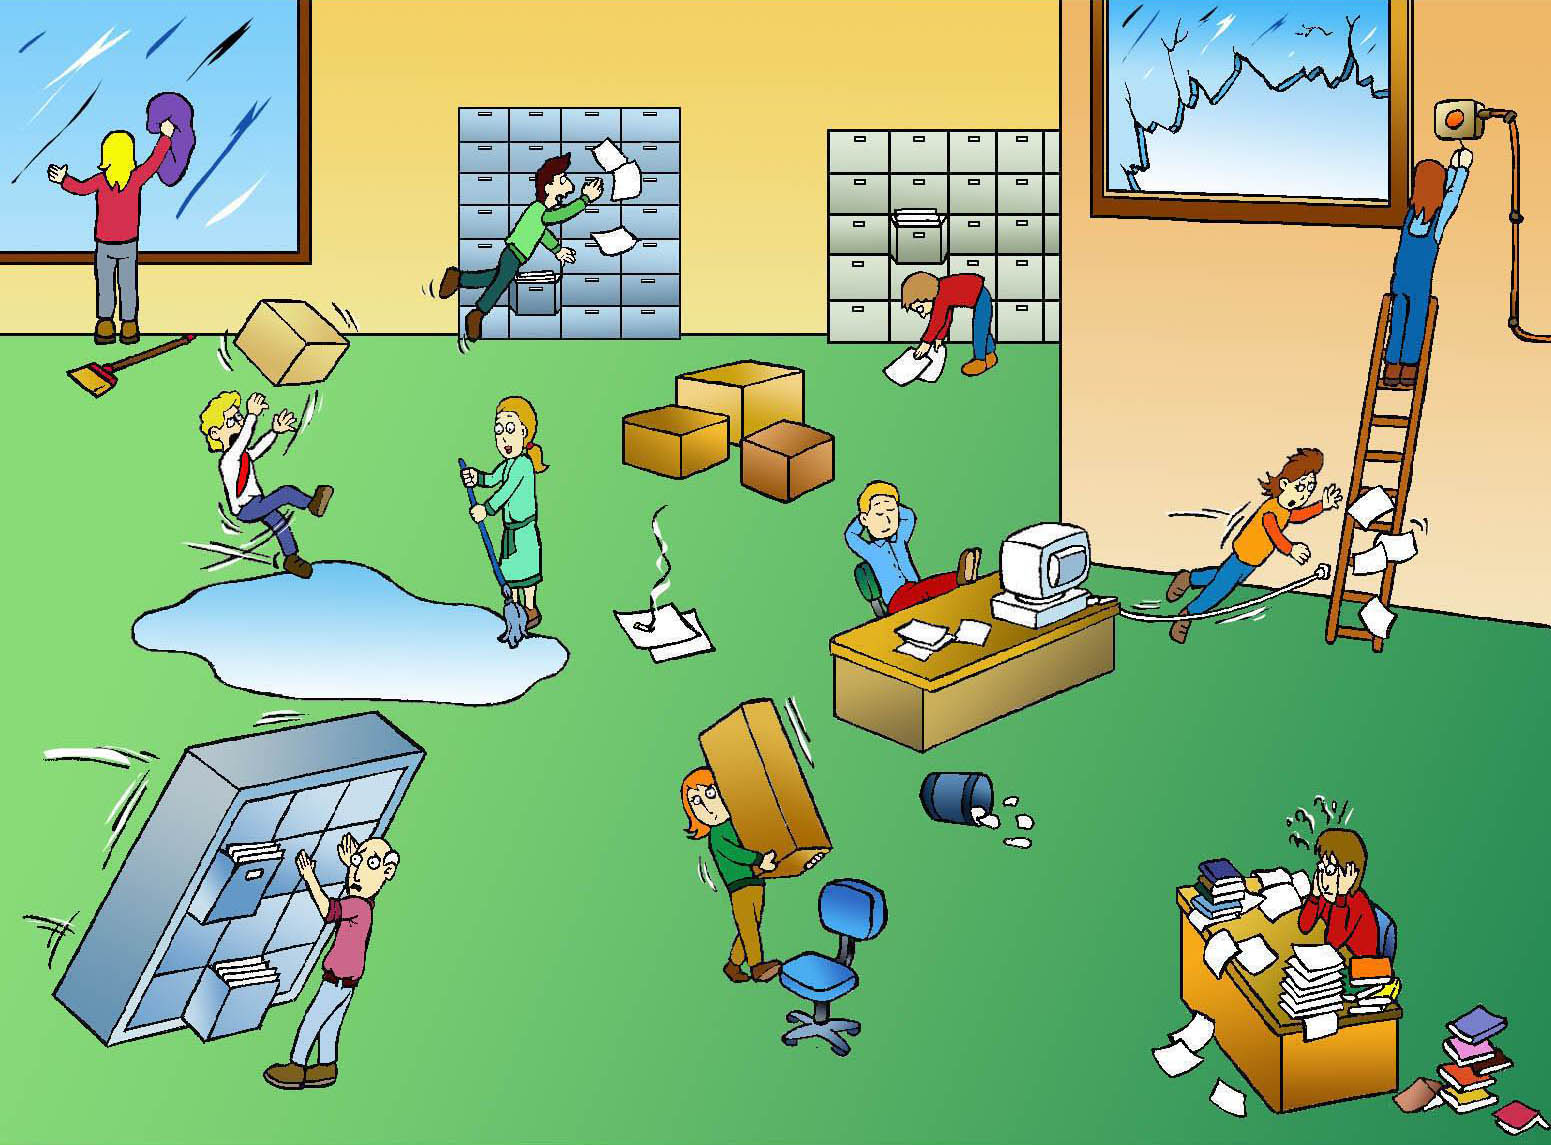
\includegraphics[width=0.9\textwidth]{../assignments/images/Identificación de Riesgos/07.jpg}
	
	\subsection{Persona 1 (Borde de estructura elevada - arriba izquierda)}
	
	\subsubsection{Riesgos Identificados}
	\begin{itemize}
		\item \textit{Caída de personas a distinto nivel:} Falta total de protección en borde de trabajo en altura.
	\end{itemize}
	
	\subsubsection{Medidas a Adoptar}
	\begin{itemize}
		\item Instalación \textbf{urgente} de protecciones colectivas: barandillas perimetrales reglamentarias (altura mín. 90cm, con listón intermedio y rodapié).
		\item Uso obligatorio de Equipos de Protección Individual (EPI) anticaídas (arnés conectado a línea de vida o punto de anclaje seguro).
		\item Señalización de riesgo de caída.
		\item Formación específica para trabajos en altura.
	\end{itemize}
	
	\subsubsection{Nivel de Riesgo}
	\begin{itemize}
		\item Caída personas distinto nivel: \textbf{Muy Alto}
	\end{itemize}
	
	\bigskip\hrulefill\bigskip
	
	\subsection{Persona 2 (Bajando escalera - arriba izquierda)}
	
	\subsubsection{Riesgos Identificados}
	\begin{itemize}
		\item \textit{Caída de personas a distinto nivel:} Escalera manual inestable, posiblemente corta, mal apoyada y sin asegurar.
		\item \textit{Caída de objetos en manipulación:} Si lleva herramientas/materiales.
		\item \textit{Golpes contra objetos inmóviles:} Al caer.
	\end{itemize}
	
	\subsubsection{Medidas a Adoptar}
	\begin{itemize}
		\item Utilizar únicamente escaleras homologadas, revisadas y en buen estado.
		\item Asegurar que la escalera sobrepasa en 1 metro el punto de desembarco.
		\item Apoyar la escalera sobre base firme y estable, con el ángulo correcto (aprox. 75º).
		\item Sujetar la escalera en la parte superior y/o inferior para evitar deslizamientos.
		\item Formación sobre uso seguro (tres puntos de apoyo, no transportar cargas).
		\item Valorar uso de medios más seguros (andamios, PEMP) para accesos habituales.
	\end{itemize}
	
	\subsubsection{Nivel de Riesgo}
	\begin{itemize}
		\item Caída personas distinto nivel: \textbf{Alto}
		\item Caída objetos manipulación: \textbf{Bajo-Medio}
		\item Golpes contra objetos inmóviles: \textbf{Bajo-Medio}
	\end{itemize}
	
	\bigskip\hrulefill\bigskip
	
	\subsection{Persona 3 (Operador de grúa - centro)}
	
	\subsubsection{Riesgos Identificados} (Genera riesgos principalmente para otros)
	\begin{itemize}
		\item \textit{Caída de objetos por desplome:} La carga suspendida (riesgo para P4, P5).
		\item \textit{Atrapamientos por o entre objetos:} Por caída o movimiento de la carga (riesgo para P4, P5).
		\item \textit{Golpes contra objetos inmóviles:} Grúa o carga contra estructuras.
		\item \textit{Contactos eléctricos:} Posible contacto con líneas eléctricas aéreas (no visibles, pero riesgo inherente).
	\end{itemize}
	
	\subsubsection{Medidas a Adoptar}
	\begin{itemize}
		\item Operador cualificado, formado y autorizado.
		\item Planificación de las maniobras de izado (plan de izado).
		\item Revisiones periódicas de la grúa, cables, ganchos y eslingas.
		\item \textbf{Prohibir y evitar} el paso o permanencia de personas bajo cargas suspendidas.
		\item Delimitar y señalizar ampliamente la zona de barrido de la carga.
		\item Verificar ausencia y mantener distancias de seguridad con líneas eléctricas.
	\end{itemize}
	
	\subsubsection{Nivel de Riesgo} (Generado para otros)
	\begin{itemize}
		\item Caída objetos / Atrapamiento: \textbf{Muy Alto} (para P4, P5)
		\item Golpes / Contacto Eléctrico: \textbf{Bajo-Medio} (aumenta si hay líneas cerca)
	\end{itemize}
	
	\bigskip\hrulefill\bigskip
	
	\subsection{Persona 4 (Bajo carga suspendida - centro, suelo)}
	
	\subsubsection{Riesgos Identificados}
	\begin{itemize}
		\item \textit{Caída de objetos por desplome / Atrapamientos por o entre objetos:} Aplastamiento por la carga de la grúa.
	\end{itemize}
	
	\subsubsection{Medidas a Adoptar}
	\begin{itemize}
		\item Nadie debe permanecer bajo cargas suspendidas.
		\item Delimitación física y señalización clara de la zona afectada por la grúa.
		\item Supervisión activa para impedir el acceso a la zona de peligro.
		\item Instrucciones claras a todo el personal sobre este riesgo.
	\end{itemize}
	
	\subsubsection{Nivel de Riesgo}
	\begin{itemize}
		\item Caída objetos / Atrapamiento: \textbf{Muy Alto}
	\end{itemize}
	
	\bigskip\hrulefill\bigskip
	
	\subsection{Persona 5 (Bajo carga suspendida - centro, suelo, cerca P4)}
	
	\subsubsection{Riesgos Identificados}
	\begin{itemize}
		\item \textit{Caída de objetos por desplome / Atrapamientos por o entre objetos:} Aplastamiento por la carga de la grúa.
	\end{itemize}
	
	\subsubsection{Medidas a Adoptar}
	\begin{itemize}
		\item Nadie debe permanecer bajo cargas suspendidas.
		\item Delimitación física y señalización clara de la zona afectada por la grúa.
		\item Supervisión activa para impedir el acceso a la zona de peligro.
		\item Instrucciones claras a todo el personal sobre este riesgo.
	\end{itemize}
	
	\subsubsection{Nivel de Riesgo}
	\begin{itemize}
		\item Caída objetos / Atrapamiento: \textbf{Muy Alto}
	\end{itemize}
	
	\bigskip\hrulefill\bigskip
	
	\subsection{Persona 6 (Usando martillo neumático en altura - derecha, arriba)}
	
	\subsubsection{Riesgos Identificados}
	\begin{itemize}
		\item \textit{Caída de personas a distinto nivel:} Trabajo cerca de borde sin protección aparente.
		\item \textit{Proyección de fragmentos o partículas:} Escombros generados.
		\item \textit{Caída de objetos por desplome:} Escombros que caen sobre P7.
		\item \textit{Sobreesfuerzos / Posturas inadecuadas:} Manejo de herramienta pesada/vibratoria.
		\item (\textit{Riesgos no listados: Ruido, Vibraciones}).
	\end{itemize}
	
	\subsubsection{Medidas a Adoptar}
	\begin{itemize}
		\item Instalar protecciones colectivas (barandillas, redes perimetrales).
		\item Uso de EPIs: sistema anticaídas, casco, gafas/pantalla facial, protección auditiva, guantes antivibración.
		\item Instalar protección inferior (marquesinas, redes) para evitar caída de objetos sobre P7.
		\item Delimitar y señalizar zona inferior.
		\item Planificar trabajos para evitar simultaneidad si no hay protección.
		\item Rotación de tareas, pausas (por vibraciones/esfuerzo).
	\end{itemize}
	
	\subsubsection{Nivel de Riesgo}
	\begin{itemize}
		\item Caída personas distinto nivel: \textbf{Alto}
		\item Caída objetos desplome (sobre P7): \textbf{Alto}
		\item Proyección fragmentos/partículas: \textbf{Medio-Alto}
		\item Sobreesfuerzos / Posturas inadecuadas: \textbf{Medio}
		\item (\textit{Ruido/Vibraciones: Alto si no hay control})
	\end{itemize}
	
	\bigskip\hrulefill\bigskip
	
	\subsection{Persona 7 (Bajo zona de demolición - derecha, abajo)}
	
	\subsubsection{Riesgos Identificados}
	\begin{itemize}
		\item \textit{Caída de objetos por desplome:} Escombros cayendo desde el trabajo de P6.
		\item \textit{Pisadas sobre objetos / Golpes contra objetos inmóviles:} Escombros en el suelo.
		\item \textit{Posturas inadecuadas:} Al agacharse sobre los escombros.
		\item \textit{Proyección de fragmentos o partículas:} Procedentes de P6 o al manipular escombros.
	\end{itemize}
	
	\subsubsection{Medidas a Adoptar}
	\begin{itemize}
		\item Prohibir trabajos simultáneos a distinta altura si no hay protección
		\item Instalar protección superior (redes, marquesinas robustas).
		\item Delimitar y señalizar la zona inferior prohibiendo el acceso.
		\item Uso obligatorio de casco con barboquejo.
		\item Orden y limpieza periódica de la zona.
	\end{itemize}
	
	\subsubsection{Nivel de Riesgo}
	\begin{itemize}
		\item Caída objetos desplome: \textbf{Alto}
		\item Pisadas / Golpes: \textbf{Medio}
		\item Posturas inadecuadas: \textbf{Medio}
		\item Proyección fragmentos/partículas: \textbf{Medio}
	\end{itemize}
	
	\bigskip\hrulefill\bigskip
	
	\subsection{Persona 8 (Transportando tubos/barras - derecha, abajo)}
	
	\subsubsection{Riesgos Identificados}
	\begin{itemize}
		\item \textit{Caída de personas al mismo nivel:} Tropiezo con desorden general (escombros).
		\item \textit{Pisadas sobre objetos:} Escombros, materiales.
		\item \textit{Sobreesfuerzos:} Por peso/longitud del material.
		\item \textit{Golpes contra objetos inmóviles:} Con los tubos contra objetos/personas, o al tropezar.
		\item \textit{Caída de objetos en manipulación:} Los tubos/barras.
	\end{itemize}
	
	\subsubsection{Medidas a Adoptar}
	\begin{itemize}
		\item Mantener las vías de circulación despejadas y ordenadas.
		\item Utilizar medios auxiliares (carretillas) si es posible.
		\item Transporte coordinado entre dos personas para cargas largas, señalizando extremos.
		\item Formación en manipulación manual de cargas.
		\item Uso de EPIs: calzado de seguridad, guantes resistentes.
	\end{itemize}
	
	\subsubsection{Nivel de Riesgo}
	\begin{itemize}
		\item Caída personas mismo nivel / Pisadas / Golpes: \textbf{Medio}
		\item Sobreesfuerzos: \textbf{Medio}
		\item Caída objetos manipulación: \textbf{Bajo-Medio}
	\end{itemize}
	
	\bigskip\hrulefill\bigskip
	
	\subsection{Persona 9 (Borde de excavación - izquierda, abajo)}
	
	\subsubsection{Riesgos Identificados}
	\begin{itemize}
		\item \textit{Caída de personas a distinto nivel:} Al interior de la excavación por cercanía al borde inestable.
		\item \textit{Caída de objetos por desplome:} Tierra/material del borde que cae sobre P10.
	\end{itemize}
	
	\subsubsection{Medidas a Adoptar}
	\begin{itemize}
		\item Mantener una distancia de seguridad respecto al borde (mín. 0.6m - 1m, o más según terreno).
		\item \textbf{Prohibir} la permanencia innecesaria cerca del borde.
		\item Señalizar y proteger el borde (vallado, barandillas si >2m profundidad).
		\item No acopiar tierra ni materiales cerca del borde de la excavación.
		\item Vigilar la estabilidad de los bordes (grietas, etc.).
	\end{itemize}
	
	\subsubsection{Nivel de Riesgo}
	\begin{itemize}
		\item Caída personas distinto nivel: \textbf{Alto}
		\item Caída objetos desplome (sobre P10): \textbf{Medio-Alto}
	\end{itemize}
	
	\bigskip\hrulefill\bigskip
	
	\subsection{Persona 10 (Dentro de excavación - izquierda, abajo)}
	
	\subsubsection{Riesgos Identificados}
	\begin{itemize}
		\item \textit{Caída de objetos por desplome / Atrapamientos por o entre objetos:} Sepultamiento por derrumbe de paredes de la zanja (sin entibar). Caída de tierra/objetos desde el borde (P9, acopios).
		\item \textit{Caída de personas a distinto nivel:} Al entrar/salir si no hay acceso seguro.
	\end{itemize}
	
	\subsubsection{Medidas a Adoptar}
	\begin{itemize}
		\item Prohibido entrar sin protección colectiva
		\item Realizar estudio geotécnico previo.
		\item Obligatoria la instalación de sistemas de contención/entibación adecuados al terreno y profundidad, o ejecución de taludes seguros.
		\item Crear accesos seguros a la zanja (escaleras, rampas).
		\item Asegurar que no hay acopios, maquinaria pesada o vibraciones cerca del borde.
		\item Uso obligatorio de casco.
		\item Vigilancia continua del estado de la excavación y presencia de agua.
		\item Permisos de trabajo específicos.
	\end{itemize}
	
	\subsubsection{Nivel de Riesgo}
	\begin{itemize}
		\item Caída objetos / Atrapamiento (Derrumbe): \textbf{Muy Alto}
		\item Caída personas distinto nivel (Acceso): \textbf{Medio}
	\end{itemize}

	
	\section{Ejercicio 8}
	
	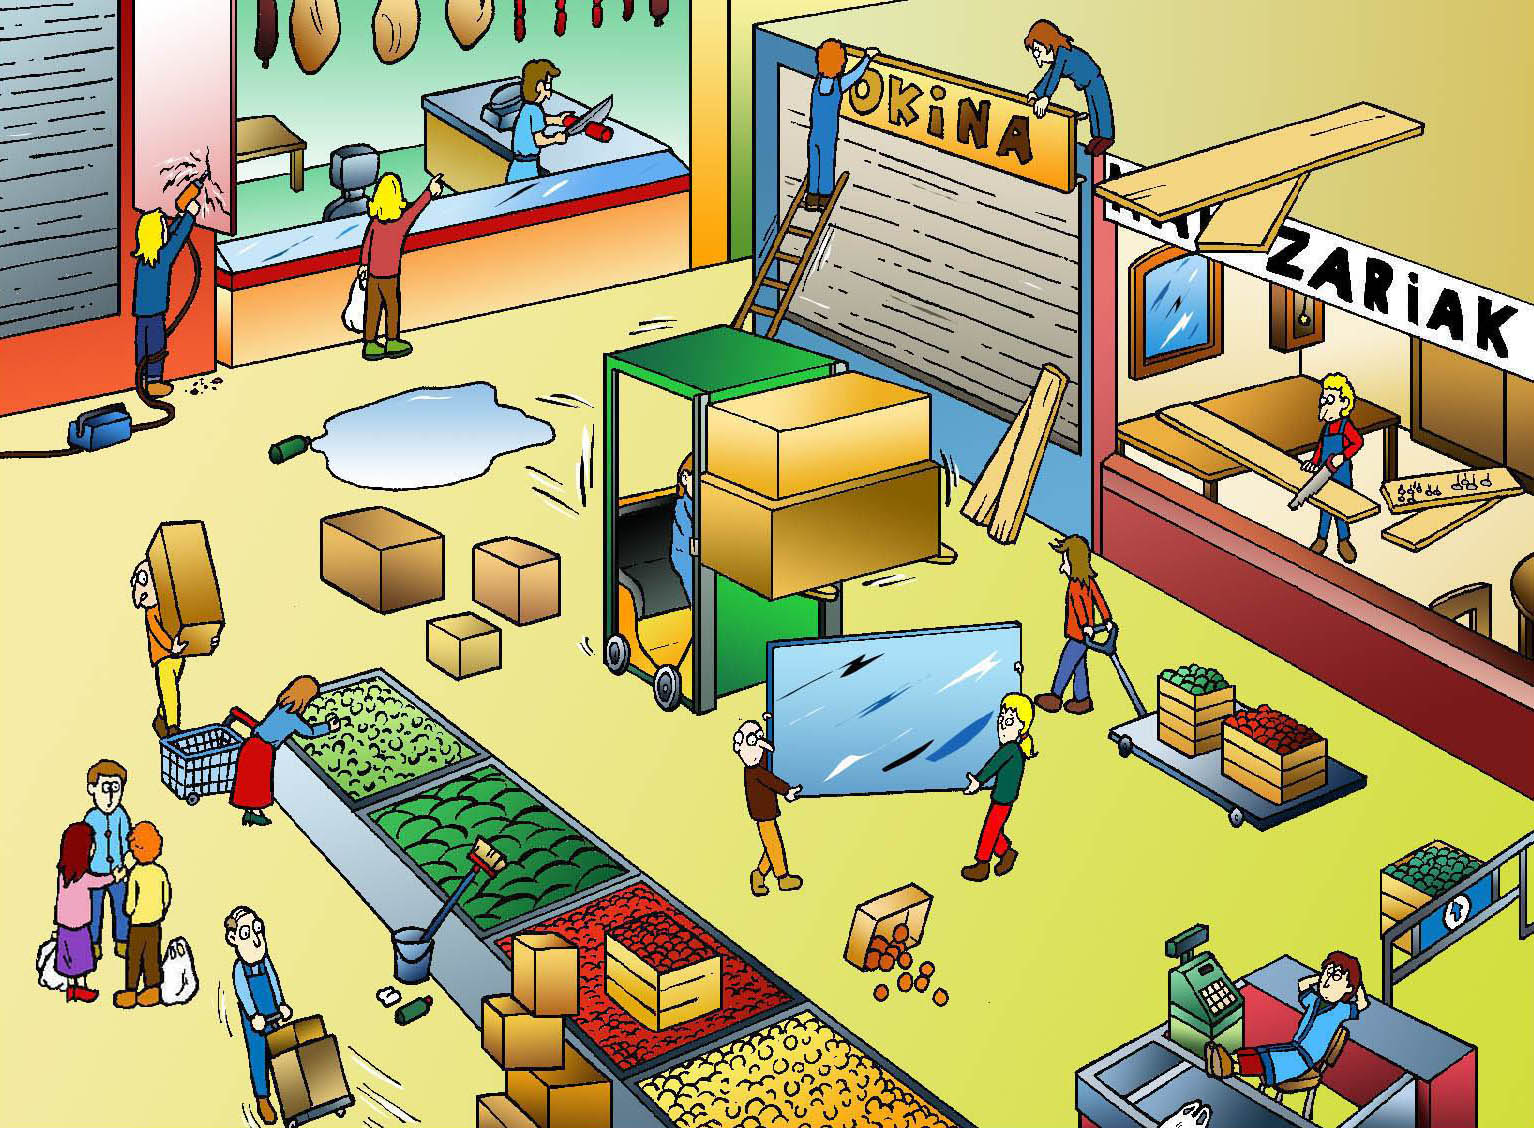
\includegraphics[width=0.9\textwidth]{../assignments/images/Identificación de Riesgos/08.jpg}
	
	\subsection{Persona 1 (Tirando de persiana - arriba izquierda)}
	
	\subsubsection{Riesgos Identificados}
	\begin{itemize}
		\item \textit{Sobreesfuerzos:} Al forzar una persiana atascada.
		\item \textit{Posturas inadecuadas:} Posición forzada al tirar.
		\item \textit{Caída de objetos por desplome:} Si la persiana cae de golpe.
		\item \textit{Atrapamientos por o entre objetos:} Con el mecanismo o la propia persiana.
	\end{itemize}
	
	\subsubsection{Medidas a Adoptar}
	\begin{itemize}
		\item No forzar mecanismos averiados; avisar a mantenimiento.
		\item Utilizar herramientas adecuadas si existen (p.ej., pértigas).
		\item Formación sobre posturas y manejo de cargas.
	\end{itemize}
	
	\subsubsection{Nivel de Riesgo}
	\begin{itemize}
		\item Sobreesfuerzos / Posturas inadecuadas: \textbf{Medio}
		\item Caída objetos desplome / Atrapamientos: \textbf{Bajo-Medio}
	\end{itemize}
	
	\bigskip\hrulefill\bigskip
	
	\subsection{Persona 2 (Carnicero/a - mostrador arriba izquierda)}
	
	\subsubsection{Riesgos Identificados}
	\begin{itemize}
		\item \textit{Caída de objetos en manipulación:} El cuchillo.
		\item \textit{Proyección de fragmentos o partículas:} Posibles esquirlas de hueso (poco probable).
		\item \textit{Posturas inadecuadas:} Dependiendo de la altura de la tabla y la tarea repetitiva.
		\item (\textit{Riesgo no listado: Cortes}).
	\end{itemize}
	
	\subsubsection{Medidas a Adoptar}
	\begin{itemize}
		\item Uso de EPIs: guante de malla en la mano no dominante, mandil.
		\item Cuchillos adecuados, bien afilados y mantenidos.
		\item Superficie de trabajo estable y a altura ergonómica.
		\item Formación específica en corte y uso seguro de herramientas.
	\end{itemize}
	
	\subsubsection{Nivel de Riesgo}
	\begin{itemize}
		\item Caída objetos manipulación / Proyección partículas / Posturas inadecuadas: \textbf{Bajo-Medio}
		\item (\textit{Riesgo de Cortes: Alto si no se usan EPIs})
	\end{itemize}
	
	\bigskip\hrulefill\bigskip
	
	\subsection{Persona 3 (Cliente/a estirándose - mostrador arriba izquierda)}
	
	\subsubsection{Riesgos Identificados}
	\begin{itemize}
		\item \textit{Caída de personas al mismo nivel:} Pérdida de equilibrio al inclinarse sobre el mostrador.
		\item \textit{Posturas inadecuadas:} Estiramiento forzado.
	\end{itemize}
	
	\subsubsection{Medidas a Adoptar}
	\begin{itemize}
		\item Diseño adecuado de mostradores para facilitar el alcance o la atención.
		\item Fomentar que los clientes pidan ayuda al personal.
	\end{itemize}
	
	\subsubsection{Nivel de Riesgo}
	\begin{itemize}
		\item Caída personas mismo nivel / Posturas inadecuadas: \textbf{Bajo}
	\end{itemize}
	
	\bigskip\hrulefill\bigskip
	
	\subsection{Persona 4 (Cargando caja, cerca derrame - centro izquierda)}
	
	\subsubsection{Riesgos Identificados}
	\begin{itemize}
		\item \textit{Caída de personas al mismo nivel:} Por el líquido derramado en el suelo.
		\item \textit{Sobreesfuerzos:} Por el peso/volumen de la caja.
		\item \textit{Caída de objetos en manipulación:} La caja.
		\item \textit{Inhalación o ingestión sustancias nocivas:} Si el derrame es de un producto químico peligroso (desconocido en la imagen).
	\end{itemize}
	
	\subsubsection{Medidas a Adoptar}
	\begin{itemize}
		\item Señalizar y limpiar \textbf{inmediatamente} cualquier derrame.
		\item Utilizar medios auxiliares (carritos) para transportar cargas.
		\item Usar calzado de trabajo con suela antideslizante.
		\item Identificar productos químicos, leer etiquetas (FDS) y usar EPIs si son necesarios al limpiar.
	\end{itemize}
	
	\subsubsection{Nivel de Riesgo}
	\begin{itemize}
		\item Caída personas mismo nivel: \textbf{Medio}
		\item Sobreesfuerzos / Caída objetos manipulación: \textbf{Bajo-Medio}
		\item Inhalación/ingestión sustancias nocivas: \textbf{Bajo} (aumentaría si se confirmara que es una sustancia peligrosa).
	\end{itemize}
	
	\bigskip\hrulefill\bigskip
	
	\subsection{Persona 5 (Grupo clientes cerca fruta - abajo izquierda)}
	
	\subsubsection{Riesgos Identificados}
	\begin{itemize}
		\item \textit{Caída de personas al mismo nivel:} Por fruta/verdura caída en el suelo.
		\item \textit{Pisadas sobre objetos:} Fruta/verdura en el suelo.
		\item \textit{Golpes contra objetos inmóviles:} Con los bordes de los expositores.
	\end{itemize}
	
	\subsubsection{Medidas a Adoptar}
	\begin{itemize}
		\item Diseño de expositores que minimice la caída de producto.
		\item Limpieza frecuente de la zona por parte del personal.
		\item Supervisión de los niños por parte de los adultos.
	\end{itemize}
	
	\subsubsection{Nivel de Riesgo}
	\begin{itemize}
		\item Caída personas mismo nivel / Pisadas sobre objetos: \textbf{Bajo-Medio}
		\item Golpes contra objetos inmóviles: \textbf{Bajo}
	\end{itemize}
	
	\bigskip\hrulefill\bigskip
	
	\subsection{Persona 6 (Cliente/a cogiendo fruta - abajo izquierda)}
	
	\subsubsection{Riesgos Identificados}
	\begin{itemize}
		\item \textit{Posturas inadecuadas:} Al agacharse o inclinarse sobre cajones bajos.
		\item \textit{Caída de personas al mismo nivel:} Por posible fruta/verdura en el suelo.
	\end{itemize}
	
	\subsubsection{Medidas a Adoptar}
	\begin{itemize}
		\item Diseño ergonómico de los expositores (altura).
		\item Limpieza frecuente del suelo.
	\end{itemize}
	
	\subsubsection{Nivel de Riesgo}
	\begin{itemize}
		\item Posturas inadecuadas: \textbf{Bajo-Medio}
		\item Caída personas mismo nivel: \textbf{Bajo}
	\end{itemize}
	
	\bigskip\hrulefill\bigskip
	
	\subsection{Persona 7 (Tirando de carro - abajo izquierda)}
	
	\subsubsection{Riesgos Identificados}
	\begin{itemize}
		\item \textit{Sobreesfuerzos:} Al tirar de un carro pesado (mayor esfuerzo que empujar).
		\item \textit{Posturas inadecuadas:} Por tirar del carro, posible torsión del tronco.
		\item \textit{Golpes contra objetos inmóviles/personas:} Menor visibilidad al tirar hacia atrás.
		\item \textit{Caída de personas al mismo nivel:} Si tropieza durante la maniobra.
	\end{itemize}
	
	\subsubsection{Medidas a Adoptar}
	\begin{itemize}
		\item \textbf{Empujar} los carros siempre que sea posible.
		\item Utilizar carros adecuados al peso, bien mantenidos (ruedas).
		\item Asegurar buena visibilidad de la ruta.
		\item Mantener pasillos despejados.
	\end{itemize}
	
	\subsubsection{Nivel de Riesgo}
	\begin{itemize}
		\item Sobreesfuerzos / Posturas inadecuadas: \textbf{Medio}
		\item Golpes / Caída personas mismo nivel: \textbf{Bajo-Medio}
	\end{itemize}
	
	\bigskip\hrulefill\bigskip
	
	\subsection{Persona 8 (Operando carretilla - centro)}
	
	\subsubsection{Riesgos Identificados}
	\begin{itemize}
		\item \textit{Atrapamientos por o entre objetos:} Para P11 (detrás) o si cae la carga.
		\item \textit{Caída de objetos por desplome:} La carga elevada y posiblemente inestable.
		\item \textit{Golpes contra objetos inmóviles/personas:} Visibilidad reducida por la carga, entorno concurrido.
		\item \textit{Caída de personas al mismo nivel:} Atropello de P11 u otros peatones/clientes.
	\end{itemize}
	
	\subsubsection{Medidas a Adoptar}
	\begin{itemize}
		\item Conductor formado y autorizado.
		\item Circular con la carga lo más baja posible.
		\item Asegurar visibilidad (espejos, ayuda si es necesario).
		\item Usar señales acústicas/luminosas en zonas de peatones.
		\item Delimitar claramente zonas de paso peatonal y de carretillas si es posible.
		\item Restringir uso de carretillas en horas de máxima afluencia de público si es viable.
		\item Prohibir situarse detrás o en puntos ciegos de la carretilla.
	\end{itemize}
	
	\subsubsection{Nivel de Riesgo}
	\begin{itemize}
		\item Atrapamientos / Golpes (para P11): \textbf{Alto}
		\item Caída objetos desplome / Golpes generales / Caída personas (atropello): \textbf{Medio}
	\end{itemize}
	
	\bigskip\hrulefill\bigskip
	
	\subsection{Persona 9 (Subiendo escalera - centro)}
	
	\subsubsection{Riesgos Identificados}
	\begin{itemize}
		\item \textit{Caída de personas a distinto nivel:} Si la escalera es inestable, está mal colocada, o si se estira demasiado lateralmente ("sobrealcance").
		\item \textit{Caída de objetos en manipulación:} El cartel ``POKINA'' o herramientas.
		\item \textit{Sobreesfuerzos / Posturas inadecuadas:} Al colocar el cartel en posición forzada.
	\end{itemize}
	
	\subsubsection{Medidas a Adoptar}
	\begin{itemize}
		\item Usar escaleras homologadas, adecuadas para la altura, revisadas y en buen estado.
		\item Colocar la escalera sobre suelo firme y nivelado, asegurando su estabilidad.
		\item No estirarse lateralmente fuera de los límites de la escalera. Mantener 3 puntos de apoyo.
		\item Subir/bajar el material de forma segura (no llevarlo en las manos al subir/bajar).
	\end{itemize}
	
	\subsubsection{Nivel de Riesgo}
	\begin{itemize}
		\item Caída personas distinto nivel: \textbf{Medio-Alto}
		\item Caída objetos manipulación / Sobreesfuerzos / Posturas: \textbf{Bajo}
	\end{itemize}
	
	\bigskip\hrulefill\bigskip
	
	\subsection{Persona 10 (Sobre estructura estrecha - arriba centro)}
	
	\subsubsection{Riesgos Identificados}
	\begin{itemize}
		\item \textit{Caída de personas a distinto nivel:} Equilibrio totalmente precario sobre una superficie mínima a una altura considerable.
	\end{itemize}
	
	\subsubsection{Medidas a Adoptar}
	\begin{itemize}
		\item Prohibición absoluta de esta práctica es un acto inseguro.
		\item Utilizar medios auxiliares seguros para trabajos en altura: andamio normalizado, plataforma elevadora móvil de personal (PEMP).
		\item Si, excepcionalmente y justificado, fuera necesario un acceso similar (que no debería), requeriría medidas extremas: línea de vida, arnés anticaídas, estudio previo, etc.
	\end{itemize}
	
	\subsubsection{Nivel de Riesgo}
	\begin{itemize}
		\item Caída personas distinto nivel: \textbf{Muy Alto}
	\end{itemize}
	
	\bigskip\hrulefill\bigskip
	
	\subsection{Persona 11 (Detrás de carretilla - centro)}
	
	\subsubsection{Riesgos Identificados}
	\begin{itemize}
		\item \textit{Atrapamientos por o entre objetos / Golpes contra objetos:} Ser golpeado/atrapado por la carretilla si retrocede, gira o frena bruscamente.
		\item \textit{Caída de personas al mismo nivel:} Ser atropellado por la carretilla.
	\end{itemize}
	
	\subsubsection{Medidas a Adoptar}
	\begin{itemize}
		\item Prohibido caminar pegado detrás o en puntos ciegos de carretillas
		\item Mantener siempre una distancia de seguridad prudencial.
		\item Intentar establecer contacto visual con el conductor.
		\item Utilizar las rutas peatonales designadas si existen.
		\item Formación/Información a todo el personal (y visible para clientes) sobre los peligros de circular cerca de carretillas.
	\end{itemize}
	
	\subsubsection{Nivel de Riesgo}
	\begin{itemize}
		\item Atrapamientos / Golpes / Caída (atropello): \textbf{Alto}
	\end{itemize}
	
	\bigskip\hrulefill\bigskip
	
	\subsection{Persona 12 y 13 (Transportando panel - centro abajo)}
	
	\subsubsection{Riesgos Identificados}
	\begin{itemize}
		\item \textit{Caída de objetos en manipulación:} El panel (¿vidrio?), que es grande, pesado y difícil de agarrar.
		\item \textit{Sobreesfuerzos / Posturas inadecuadas:} Por el peso, volumen y agarre incómodo.
		\item \textit{Golpes contra objetos inmóviles/personas:} Dificultad de visión periférica y maniobrabilidad reducida.
		\item \textit{Caída de personas al mismo nivel:} Tropiezo durante el transporte.
		\item (\textit{Riesgo no listado: Cortes si es vidrio y rompe}).
	\end{itemize}
	
	\subsubsection{Medidas a Adoptar}
	\begin{itemize}
		\item Utilizar medios auxiliares: carros específicos para paneles/vidrio, ventosas de transporte si aplica.
		\item Planificar la ruta, despejarla de obstáculos y señalizar si es necesario.
		\item Coordinación entre las dos personas.
		\item Uso de EPIs: guantes de agarre (y anticorte si es vidrio), calzado de seguridad.
	\end{itemize}
	
	\subsubsection{Nivel de Riesgo}
	\begin{itemize}
		\item Caída objeto manipulación / Sobreesfuerzos / Posturas: \textbf{Medio-Alto}
		\item Golpes / Caída personas mismo nivel: \textbf{Medio}
		\item (\textit{Cortes: Alto si es vidrio y no usan EPIs})
	\end{itemize}
	
	\bigskip\hrulefill\bigskip
	
	\subsection{Persona 14 (Instalando estantería - derecha)}
	
	\subsubsection{Riesgos Identificados}
	\begin{itemize}
		\item \textit{Caída de objetos por desplome:} Partes de la estantería durante el montaje, tablones cercanos mal apoyados.
		\item \textit{Golpes contra objetos inmóviles:} Con herramientas, partes de la estantería, tablones.
		\item \textit{Posturas inadecuadas / Sobreesfuerzos:} Al manipular piezas, agacharse, levantar peso.
		\item \textit{Proyección de fragmentos o partículas:} Si usa taladro u otras herramientas.
		\item \textit{Pisadas sobre objetos:} Herramientas, piezas o embalajes dejados en el suelo.
	\end{itemize}
	
	\subsubsection{Medidas a Adoptar}
	\begin{itemize}
		\item Asegurar la estabilidad provisional de los componentes durante el montaje.
		\item Mantener la zona de trabajo ordenada y despejada.
		\item Seguir instrucciones de montaje. Utilizar posturas adecuadas.
		\item Uso de EPIs según la herramienta (gafas si hay proyección).
	\end{itemize}
	
	\subsubsection{Nivel de Riesgo}
	\begin{itemize}
		\item Caída objetos desplome / Golpes / Posturas / Sobreesfuerzos: \textbf{Medio}
		\item Proyección partículas / Pisadas: \textbf{Bajo-Medio}
	\end{itemize}
	
	\bigskip\hrulefill\bigskip
	
	\subsection{Persona 15 (Cajero/a - abajo derecha)}
	
	\subsubsection{Riesgos Identificados}
	\begin{itemize}
		\item \textit{Posturas inadecuadas:} Por diseño no ergonómico del puesto (asiento inadecuado, altura incorrecta de pantalla/scaner, espacio insuficiente). Movimientos repetitivos.
		\item \textit{Sobreesfuerzos:} Al manipular productos pesados o voluminosos de los clientes.
	\end{itemize}
	
	\subsubsection{Medidas a Adoptar}
	\begin{itemize}
		\item Realizar evaluación ergonómica del puesto de trabajo.
		\item Proporcionar silla ergonómica ajustable.
		\item Ajustar altura de equipos. Asegurar espacio suficiente para piernas.
		\item Fomentar pausas activas y posible rotación de tareas.
		\item Formación en higiene postural y manejo de cargas.
	\end{itemize}
	
	\subsubsection{Nivel de Riesgo}
	\begin{itemize}
		\item Posturas inadecuadas: \textbf{Medio} (por exposición prolongada)
		\item Sobreesfuerzos: \textbf{Bajo-Medio}
	\end{itemize}
	
	\section{Ejercicio 9}
	
	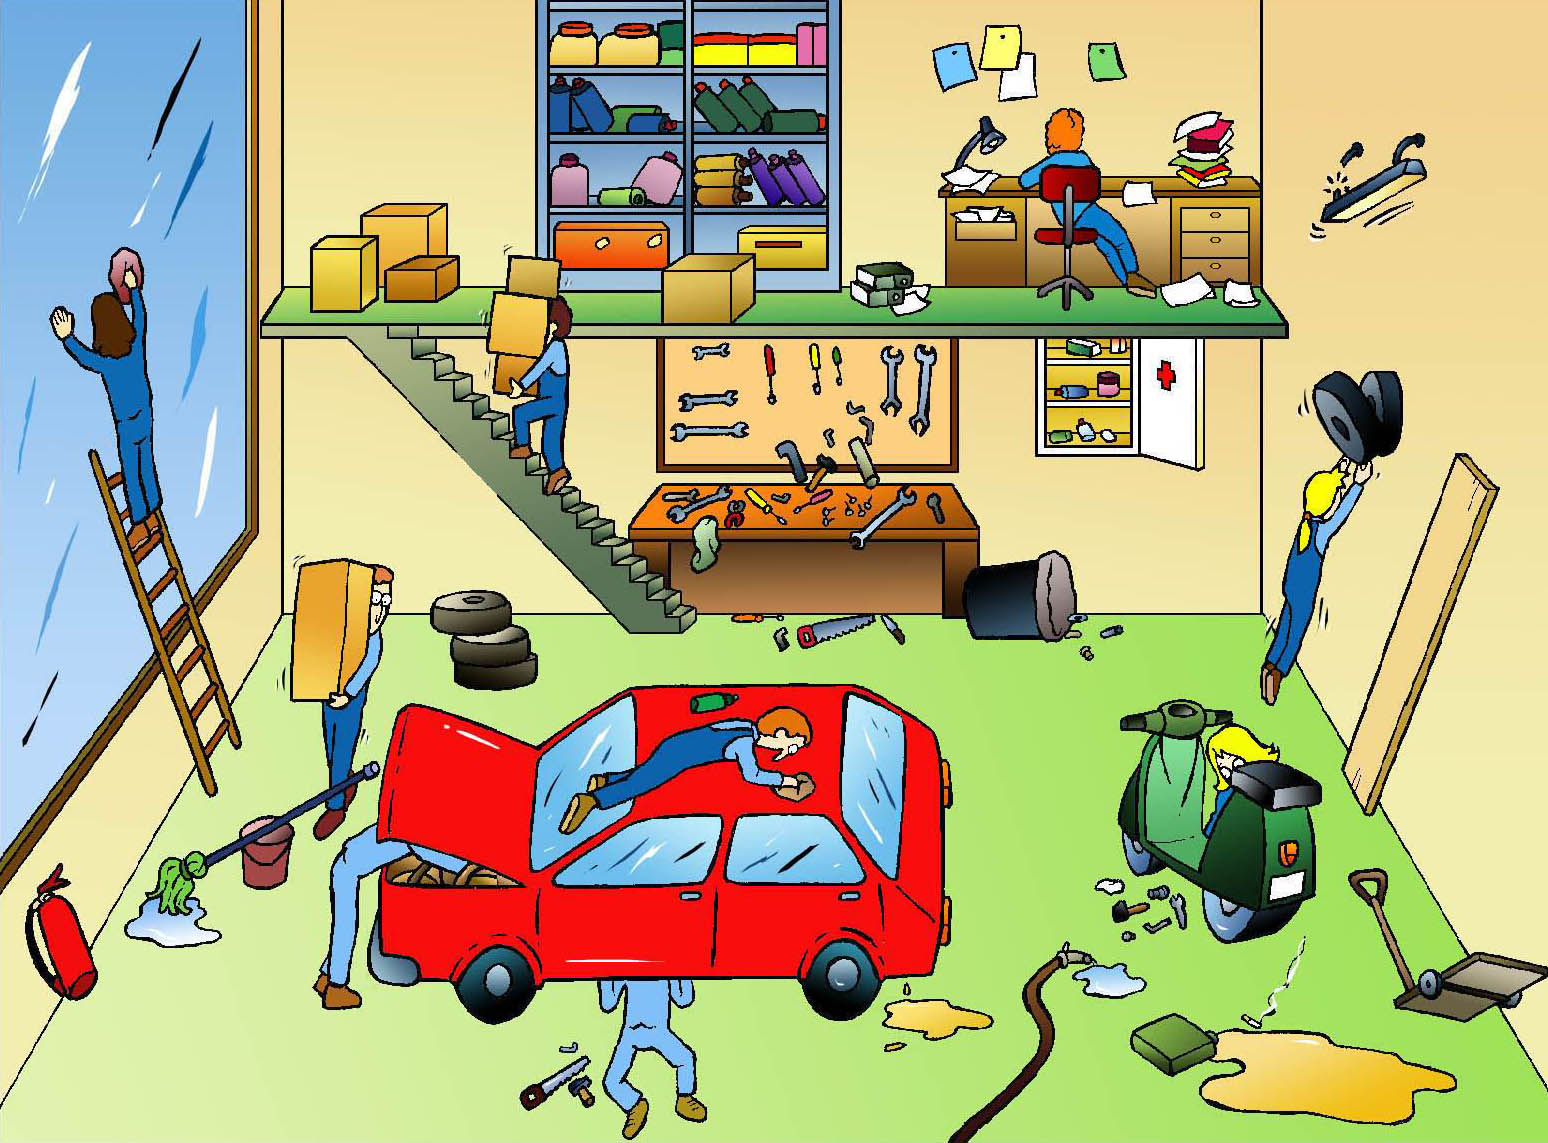
\includegraphics[width=0.9\textwidth]{../assignments/images/Identificación de Riesgos/09.jpg}
	
	\subsection{Persona 1 (Limpiando ventana en escalera - izquierda)}
	
	\subsubsection{Riesgos Identificados}
	\begin{itemize}
		\item \textit{Caída de personas a distinto nivel:} Uso de escalera manual con sobrealcance lateral.
		\item \textit{Caída de objetos en manipulación:} Útiles de limpieza (cubo, etc.).
	\end{itemize}
	
	\subsubsection{Medidas a Adoptar}
	\begin{itemize}
		\item Utilizar escalera adecuada, estable y bien posicionada. No estirarse fuera de los límites seguros.
		\item Valorar uso de plataformas o herramientas con mango extensible.
		\item Asegurar útiles de limpieza para evitar su caída.
	\end{itemize}
	
	\subsubsection{Nivel de Riesgo}
	\begin{itemize}
		\item Caída personas distinto nivel: \textbf{Alto}
		\item Caída objetos manipulación: \textbf{Bajo}
	\end{itemize}
	
	\bigskip\hrulefill\bigskip
	
	\subsection{Persona 2 (Subiendo caja por escalera - centro)}
	
	\subsubsection{Riesgos Identificados}
	\begin{itemize}
		\item \textit{Caída de personas a distinto nivel:} Dificultad de visibilidad y agarre en escalera por la carga.
		\item \textit{Caída de objetos en manipulación:} La caja transportada.
		\item \textit{Sobreesfuerzos / Posturas inadecuadas:} Al subir la carga por las escaleras.
	\end{itemize}
	
	\subsubsection{Medidas a Adoptar}
	\begin{itemize}
		\item Evaluar uso de medios mecánicos o ayuda para subir cargas.
		\item Asegurar buena visibilidad y agarre firme de la barandilla.
		\item Formación en manipulación manual de cargas y transporte en escaleras.
	\end{itemize}
	
	\subsubsection{Nivel de Riesgo}
	\begin{itemize}
		\item Caída personas distinto nivel: \textbf{Alto}
		\item Caída objetos manipulación / Sobreesfuerzos / Posturas inadecuadas: \textbf{Medio}
	\end{itemize}
	
	\bigskip\hrulefill\bigskip
	
	\subsection{Persona 3 (Oficina altillo - arriba centro)}
	
	\subsubsection{Riesgos Identificados}
	\begin{itemize}
		\item \textit{Posturas inadecuadas:} Posible riesgo ergonómico por trabajo en puesto de oficina.
		\item \textit{Caída de personas al mismo nivel:} Tropiezo con cable telefónico extendido por el suelo.
	\end{itemize}
	
	\subsubsection{Medidas a Adoptar}
	\begin{itemize}
		\item Evaluar ergonómicamente el puesto (silla, mesa, pantalla). Fomentar pausas.
		\item Organizar y fijar el cableado para evitar tropiezos.
	\end{itemize}
	
	\subsubsection{Nivel de Riesgo}
	\begin{itemize}
		\item Posturas inadecuadas: \textbf{Bajo-Medio}
		\item Caída personas mismo nivel: \textbf{Bajo}
	\end{itemize}
	
	\bigskip\hrulefill\bigskip
	
	\subsection{Persona 4 (Altillo, alcanzando estantería - arriba centro)}
	
	\subsubsection{Riesgos Identificados}
	\begin{itemize}
		\item \textit{Caída de personas a distinto nivel:} Probablemente subido/a en objeto inestable (silla, caja) para ganar altura.
		\item \textit{Caída de objetos por desplome:} Objetos almacenados en la estantería superior.
		\item \textit{Posturas inadecuadas / Sobreesfuerzos:} Al estirarse para alcanzar objetos.
	\end{itemize}
	
	\subsubsection{Medidas a Adoptar}
	\begin{itemize}
		\item Utilizar \textbf{siempre} escaleras o taburetes homologados y estables.
		\item Organizar almacenamiento: objetos pesados/frecuentes en zonas accesibles.
		\item No sobrecargar estanterías.
	\end{itemize}
	
	\subsubsection{Nivel de Riesgo}
	\begin{itemize}
		\item Caída personas distinto nivel: \textbf{Alto}
		\item Caída objetos desplome: \textbf{Medio}
		\item Posturas inadecuadas / Sobreesfuerzos: \textbf{Bajo-Medio}
	\end{itemize}
	
	\bigskip\hrulefill\bigskip
	
	\subsection{Persona 5 (Bajo el coche - centro abajo)}
	
	\subsubsection{Riesgos Identificados}
	\begin{itemize}
		\item \textit{Atrapamientos por o entre objetos / Caída de objetos por desplome:} Aplastamiento si fallan los soportes (gato) del coche.
		\item \textit{Posturas inadecuadas:} Posición tumbada prolongada, movimientos forzados.
		\item \textit{Golpes contra objetos inmóviles:} Con partes bajas del vehículo.
		\item \textit{Inhalación o ingestión sustancias nocivas:} Posibles vapores de fluidos (aceite, combustible, etc.).
	\end{itemize}
	
	\subsubsection{Medidas a Adoptar}
	\begin{itemize}
		\item Utilizar borriquetas/caballetes homologados y adecuados bajo puntos de apoyo resistentes, además del gato. Nunca trabajar solo bajo el coche sostenido únicamente por el gato.
		\item Preferir el uso de foso o elevador si está disponible.
		\item Asegurar buena ventilación de la zona.
		\item Utilizar EPIs adecuados si se manipulan fluidos (guantes, gafas).
	\end{itemize}
	
	\subsubsection{Nivel de Riesgo}
	\begin{itemize}
		\item Atrapamientos / Caída objetos desplome: \textbf{Muy Alto}
		\item Posturas inadecuadas / Inhalación sustancias: \textbf{Medio}
		\item Golpes contra objetos inmóviles: \textbf{Bajo}
	\end{itemize}
	
	\bigskip\hrulefill\bigskip
	
	\subsection{Persona 6 (En el motor - centro)}
	
	\subsubsection{Riesgos Identificados}
	\begin{itemize}
		\item \textit{Posturas inadecuadas:} Inclinación prolongada sobre el vano motor.
		\item \textit{Golpes contra objetos inmóviles:} Con el capó, motor, componentes.
		\item \textit{Contactos térmicos:} Si el motor o componentes cercanos están calientes.
		\item \textit{Atrapamientos por o entre objetos:} Con partes móviles (ventilador, correas si arranca) o por caída del capó.
	\end{itemize}
	
	\subsubsection{Medidas a Adoptar}
	\begin{itemize}
		\item Utilizar plataformas o escalones para mejorar la postura si es necesario.
		\item Asegurar firmemente la varilla de sujeción del capó.
		\item Desconectar la batería antes de intervenir cerca de partes móviles.
		\item Esperar enfriamiento o usar protección si hay riesgo térmico.
	\end{itemize}
	
	\subsubsection{Nivel de Riesgo}
	\begin{itemize}
		\item Posturas inadecuadas / Golpes / Atrapamientos: \textbf{Medio}
		\item Contactos térmicos: \textbf{Bajo-Medio}
	\end{itemize}
	
	\bigskip\hrulefill\bigskip
	
	\subsection{Persona 7 (Levantando caja - centro izquierda)}
	
	\subsubsection{Riesgos Identificados}
	\begin{itemize}
		\item \textit{Sobreesfuerzos / Posturas inadecuadas:} Al levantar carga desde el suelo.
		\item \textit{Caída de objetos en manipulación:} La caja.
	\end{itemize}
	
	\subsubsection{Medidas a Adoptar}
	\begin{itemize}
		\item Aplicar técnica correcta de levantamiento manual (doblar rodillas, espalda recta).
		\item Evitar giros del tronco con la carga.
		\item Utilizar medios auxiliares si la carga es pesada/voluminosa.
	\end{itemize}
	
	\subsubsection{Nivel de Riesgo}
	\begin{itemize}
		\item Sobreesfuerzos / Posturas inadecuadas: \textbf{Medio}
		\item Caída objetos manipulación: \textbf{Bajo}
	\end{itemize}
	
	\bigskip\hrulefill\bigskip
	
	\subsection{Persona 8 (Junto a scooter - derecha abajo)}
	
	\subsubsection{Riesgos Identificados}
	\begin{itemize}
		\item \textit{Caída de personas al mismo nivel:} Líquido derramado (aceite?), herramientas en el suelo.
		\item \textit{Pisadas sobre objetos:} Herramientas dispersas.
		\item \textit{Incendios:} Líquido inflamable derramado cerca de posibles fuentes de ignición (chispas, electricidad).
		\item \textit{Inhalación o ingestión sustancias nocivas:} Vapores del derrame (gasolina, aceite), contacto dérmico.
		\item \textit{Contactos eléctricos:} Posible uso de herramientas eléctricas cerca del derrame o con cables defectuosos.
	\end{itemize}
	
	\subsubsection{Medidas a Adoptar}
	\begin{itemize}
		\item Limpiar \textbf{inmediatamente} derrames con material absorbente adecuado.
		\item Mantener la zona de trabajo ordenada (herramientas en su sitio).
		\item Utilizar bandejas para recoger fluidos. Buena ventilación.
		\item Evitar fuentes de ignición cerca de inflamables. Revisar herramientas eléctricas.
		\item Usar guantes para manipular aceites/combustibles.
	\end{itemize}
	
	\subsubsection{Nivel de Riesgo}
	\begin{itemize}
		\item Incendios: \textbf{Medio-Alto}
		\item Caída personas mismo nivel / Pisadas / Inhalación sustancias: \textbf{Medio}
		\item Contactos eléctricos: \textbf{Bajo-Medio}
	\end{itemize}
	
	\bigskip\hrulefill\bigskip
	
	\subsection{Persona 9 (Manipulando neumáticos - derecha)}
	
	\subsubsection{Riesgos Identificados}
	\begin{itemize}
		\item \textit{Sobreesfuerzos / Posturas inadecuadas:} Por el peso y manejo de neumáticos.
		\item \textit{Caída de objetos por desplome:} Neumáticos mal apilados, tabla de madera inestable.
		\item \textit{Caída de personas al mismo nivel:} Tropiezo con neumáticos o la tabla.
		\item \textit{Golpes contra objetos inmóviles:} Con los neumáticos o la tabla.
	\end{itemize}
	
	\subsubsection{Medidas a Adoptar}
	\begin{itemize}
		\item Formación en manipulación de cargas (técnicas para neumáticos).
		\item Almacenamiento estable y ordenado de neumáticos.
		\item Retirar elementos inestables (tabla) y mantener zona despejada.
	\end{itemize}
	
	\subsubsection{Nivel de Riesgo}
	\begin{itemize}
		\item Sobreesfuerzos / Posturas inadecuadas / Caída objetos desplome: \textbf{Medio}
		\item Caída personas mismo nivel / Golpes: \textbf{Bajo-Medio}
	\end{itemize}
	
\end{document}
